\documentclass[oneside, 11pt]{article}

\usepackage[T1]{fontenc}
\usepackage[utf8]{inputenc}
\usepackage[english]{babel}
\usepackage{enumerate}
\usepackage{isotope}


\usepackage{fouriernc}
\usepackage[detect-all, binary-units, separate-uncertainty=true,
            per-mode=symbol, retain-explicit-plus, retain-unity-mantissa=false]{siunitx}

\usepackage{setspace}
\setstretch{1.2}

\setlength{\parskip}{\smallskipamount}
\setlength{\parindent}{0pt}

\usepackage[headheight=14pt]{geometry}
\geometry{marginparwidth=0.5cm, verbose, a4paper, tmargin=3cm, bmargin=3cm,
          lmargin=2cm, rmargin=2cm}

\usepackage{float}

\usepackage[fleqn]{amsmath}
\numberwithin{equation}{section}
\numberwithin{figure}{section}

\usepackage{graphicx}
\graphicspath{{images/}{../../../images/}}

\usepackage{tikz}
\usetikzlibrary{shapes}
\usetikzlibrary{plotmarks}

\newcounter{Exercise}
\setcounter{Exercise}{1}
\usepackage{xcolor}
\definecolor{shadecolor}{gray}{0.9}
\usepackage{framed}
\usepackage{caption}

\usepackage{url}


\usepackage{fancyhdr}
\pagestyle{fancy}
\fancyhf{}
\rhead{\thepage}
\renewcommand{\footrulewidth}{0pt}
\renewcommand{\headrulewidth}{0pt}

\fancypagestyle{firststyle}
{
    \fancyhf{}
    \rhead{\thepage}
    \cfoot{\includegraphics[height=30pt]{HiSPARClogo}}
    \rfoot{\includegraphics[height=25pt]{CCbysa}}
    \lfoot{
\includegraphics[height=30pt]{NIKHEFlogo}}
    \renewcommand{\footskip}{50pt}
    \renewcommand{\footrulewidth}{0.1pt}
    \renewcommand{\headrulewidth}{0pt}
}

\newcommand{\figref}[1]{Figuur~\ref{#1}}

\newcommand{\hisparc}{\textsmaller{HiSPARC}\xspace}
\newcommand{\kascade}{\textsmaller{KASCADE}\xspace}
\newcommand{\sapphire}{\textsmaller{SAPPHiRE}\xspace}
\newcommand{\jsparc}{\textsmaller{jSparc}\xspace}
\newcommand{\hdf}{\textsmaller{HDF5}\xspace}
\newcommand{\aires}{\textsmaller{AIRES}\xspace}
\newcommand{\csv}{\textsmaller{CSV}\xspace}
\newcommand{\python}{\textsmaller{PYTHON}\xspace}
\newcommand{\corsika}{\textsmaller{CORSIKA}\xspace}
\newcommand{\labview}{\textsmaller{LabVIEW}\xspace}
\newcommand{\daq}{\textsmaller{DAQ}\xspace}
\newcommand{\adc}{\textsmaller{ADC}\xspace}
\newcommand{\hi}{\textsc{h i}\xspace}
\newcommand{\hii}{\textsc{h ii}\xspace}
\newcommand{\mip}{\textsmaller{MIP}\xspace}
\newcommand{\hisparcii}{\textsmaller{HiSPARC II}\xspace}
\newcommand{\hisparciii}{\textsmaller{HiSPARC III}\xspace}

\DeclareSIUnit{\electronvolt}{\ensuremath{\mathrm{e\!\!\:V}}}

\DeclareSIUnit{\unitsigma}{\ensuremath{\sigma}}
\DeclareSIUnit{\mip}{\textsmaller{MIP}}
\DeclareSIUnit{\adc}{\textsmaller{ADC}}

\DeclareSIUnit{\gauss}{G}
\DeclareSIUnit{\parsec}{pc}
\DeclareSIUnit{\year}{yr}





%document details
\author{N.G. Schultheiss \\ translated and adapted by K. Schadenberg}
\date{}
\title{van der Waals \& Wilson}


\begin{document}
\maketitle

\section{Introduction}
There are various ways to detect and measure particles. This module will discuss two of them, the bubble chamber and the cloud chamber (also known as the Wilson chamber). Both use phase transition of a liquid to a gas or vice versa to track particles. In the next module `Cosmic Radiation' we will show how these and other detectors were used in early particle physics experiments.

Johannes Diderik van der Waals was a Dutch theoretical physicist most famous for his work on the equations of state for gases and liquids. Charles Thomson Rees Wilson was a Scottish meteorologist who tried to create clouds in sealed chambers. During his research he found that cosmic radiation could be made visible with his chambers.

\section{van der Waals}
van der Waals obtained his doctorate for his research into gas and liquid states. His dissertation was titled `Over de continuteit van den gas- en vloeistoftoestand', \textit{on the continuity of the gas and liquid state}. For this and later work he received the Nobel prize in 1910. When van der Waals was conducting his research the scientific community was not in agreement about the basic building blocks of matter. Atoms and molecules were familiar terms and accepted as fact by most chemist. But a number of well respected physicist, such as Boltzmann and Maxwell, saw molecules as little more than a convenient way of performing calculations.

The ideal gas law was known at the time in similar forms as we know today:
\begin{equation}
pV=nRT \label{eq:ideal_gas_law}
\end{equation}
The law combined the `combined gas laws' of Charles's law, Boyle's law, and Gay-Lussac's law with Avogadro's law. $p$ is the pressure of the gas, most commonly denoted in Newtons per metre squared which is the same as Pascal\footnote{Other units are also possible but this will in turn change the unit of the gas constant.}, $V$ is the volume of the gas in cubic metres (m$^3$), $T$ temperature in Kelvin (K), $n$ the amount of gas in moles (mol), and $R$ the (universal or ideal) gas constant.

van der Waals expanded upon the known gas laws using two of his own ideas:
\begin{itemize}
\item Particles in a gas occupy a finite amount of space,\\
and
\item Particles in a gas exert a force upon each other.
\end{itemize}
These two concepts were not incorporated into the ideal gas law. Because the particles inside the gas have a certain volume, the total volume into which the gas can expand decreases. The second point introduces an `adhesive force' between the atoms or molecules, increasing the pressure. The resulting pressure inside the gas will therefore be higher than one measures outside the gas. The adhesive force later became known as the van der Waals force and is now widely used in chemistry, not only for gases.

Adding these changes to the ideal gas law results in the van der Waals equation:
\begin{equation}
\left( p+ \frac{n^{2} a}{V^2} \right) \left( V -nB \right)  = nRT \label{eq:vdw_1}
\end{equation}
$a$ is the measure of attraction between the particles and $b$ is the volume excluded by one mole of particles. We can rewrite equation~\ref{eq:vdw_1} into
\begin{equation}
p=\frac{nRT}{V-nb}-\frac{n^{2}a}{V^2}
\end{equation}
if one wants to obtain the pressure.

The values for $a$ and $b$ are different for each gas or liquid and can be determined using the critical properties of the fluid. A complete derivation is beyond the scope of this text. We will simply state the values for water: $a=0.55~\frac{\mbox{Nm}^4}{\mbox{mol}^2}$ and $b=30.4 \cdot 10^{-6}~\frac{\mbox{m}^3}{\mbox{mol}}$.

In figure~\ref{fig:vdw0} the results from equation~\ref{eq:vdw_1} for different temperatures are shown. Where the ideal gas law would show a simple monotonically falling dependence between pressure and volume, the van der Waals equations shows oscillations at certain temperatures. Only above the critical temperature does it follow the ideal gas law. When a gas follows the ideal gas law we call this gas an ideal gas. Below the critical temperature a change of phase, from liquid to gas or reverse, can be observed when changing the pressure or volume. With an ideal gas this would not happen.

Where this change of phase occurs can be calculated using Maxwell's equal area rule. This rule states that there is a certain saturation pressure of the gas. This pressure can be found by drawing a line in the graph in such a way that the area above and below in line, inside the oscillation, are equal, as shown in figure~\ref{fig:vdw0}. Inside this area both the liquid and gas phase occur. 

\begin{figure}\begin{center}
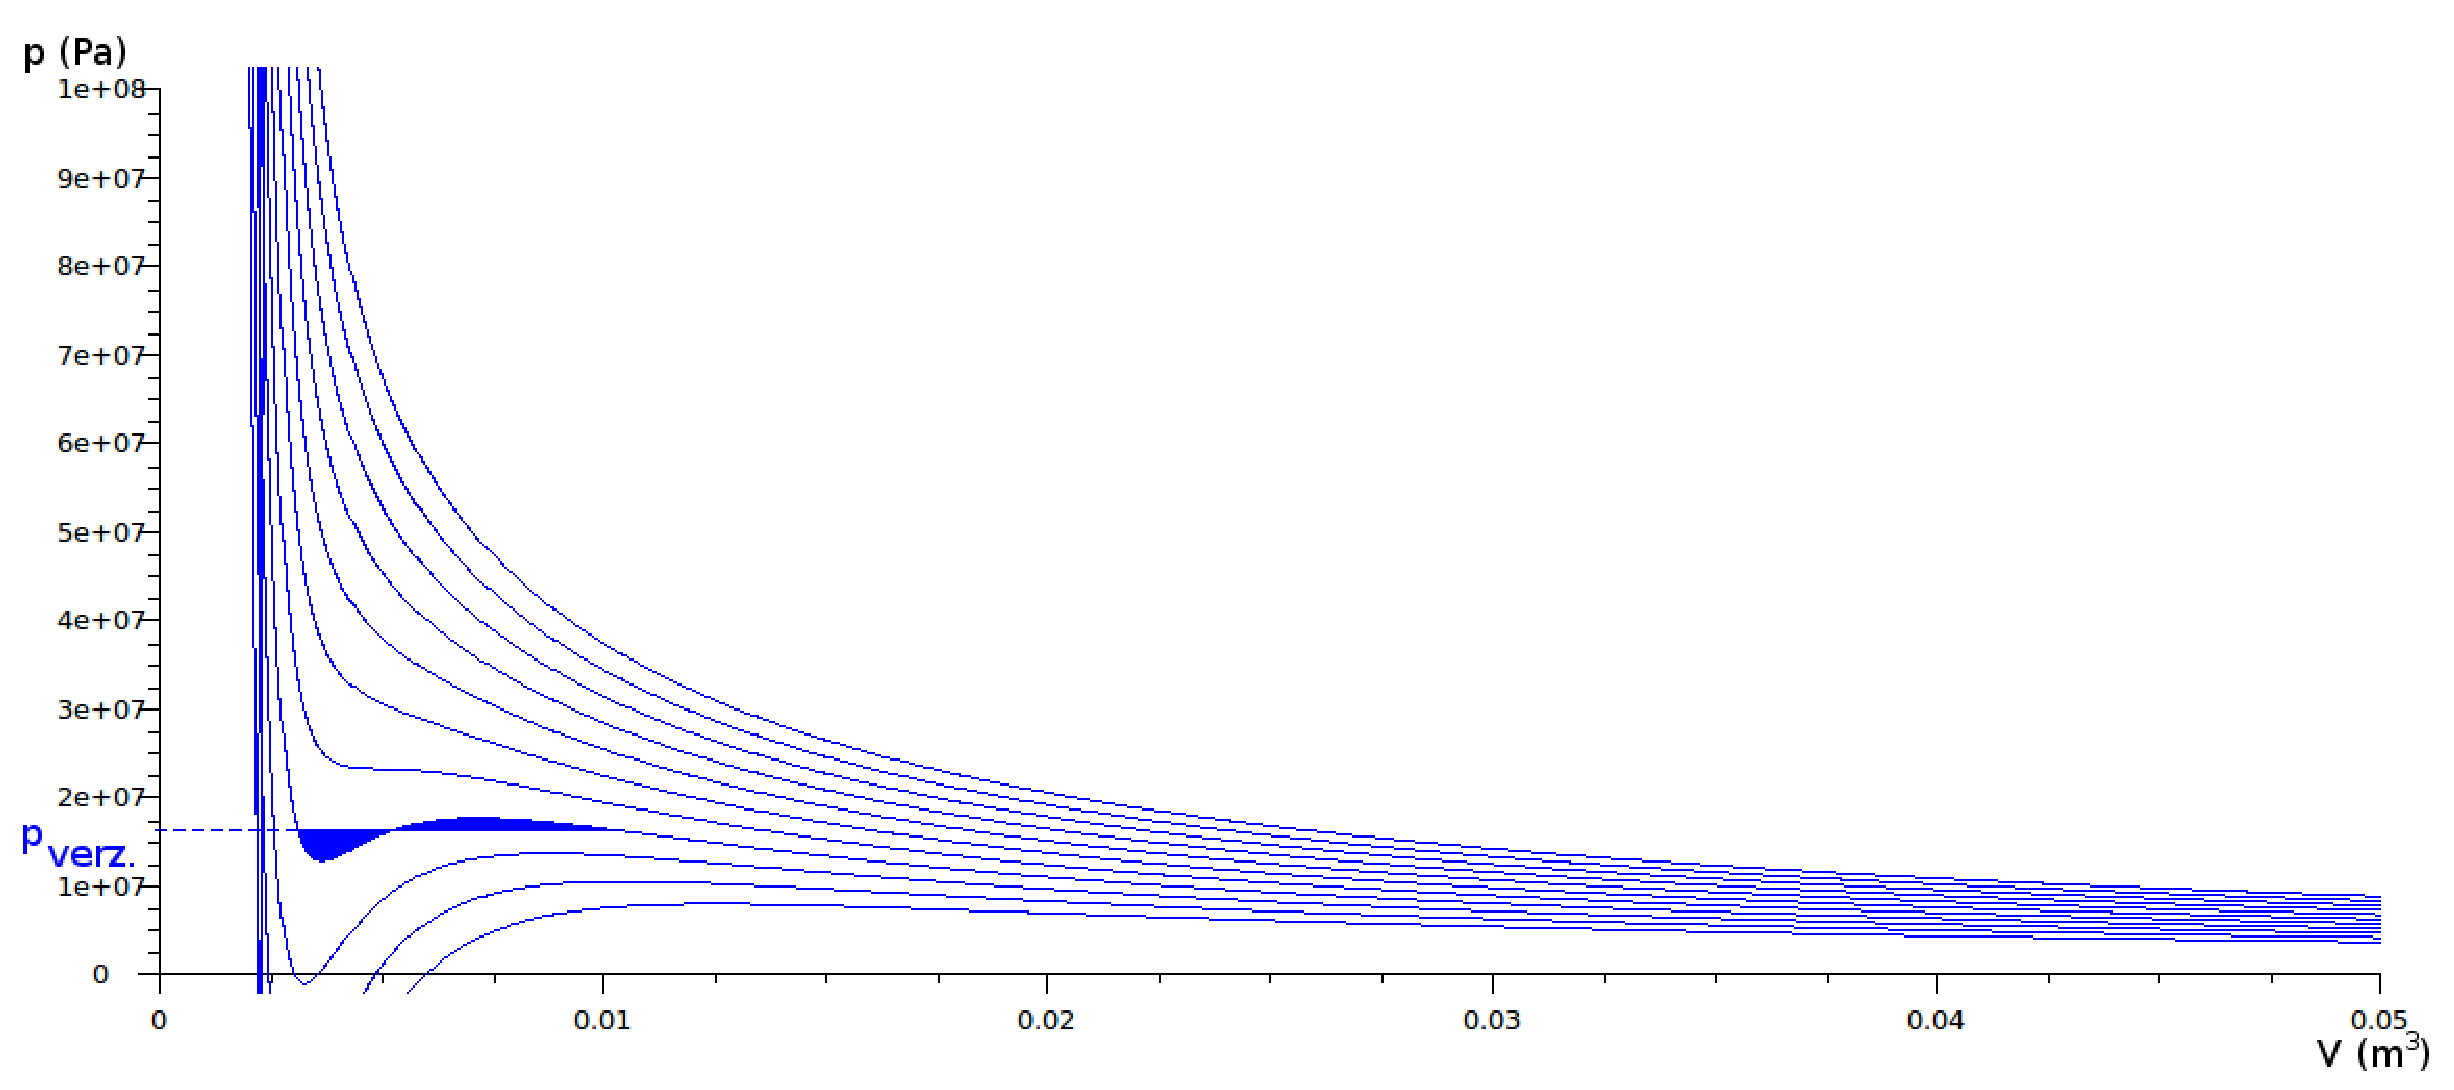
\includegraphics[scale=0.38]{vdwaals0.eps}%
\caption{The dependence of pressure and volume with differing temperatures.}\label{fig:vdw0}
\end{center}\end{figure}

When we expand the fluid we descend from the liquid phase (left hand side of the graph) until the saturation pressure is reached. If the expansion is rapid enough and we have a pure liquid it is possible to reach pressures below the saturation pressure. We then have a superheated liquid. The liquid wants to boil, but is unable to. When the smallest disturbance passes through the liquid, such as an ionizing particle, a stream of gas bubble will appear.\footnote{This is also why you add boiling chips or stones to a liquid when you heat it in a test tube, to prevent super heating.}

With a slow expansion of the volume the pressure will rise up to the saturation pressure. In a pure fluid, free from contaminants and dust, it is possible to reach pressures below the saturation pressure. When this happens we have a supersaturated vapour. When a dust or ionizing particle passes through the vapour the gas around it will immediately condense into liquid, leaving behind a streak of small droplets. This is the starting point for a cloud chamber.

Obtaining the supersaturated vapour for the cloud chamber can also be done in a different way, by quickly expanding the volume and allowing the liquid/gas to cool down. The sudden and large drop in temperature will also yield a supersaturated vapour.

A third way of making a cloud chamber makes use of diffusion. In this type of chamber there is a constant exchange of vapour between a hot and a cold environment. The vapour will condense when it enters the cold environment. In this cold environment there is a constant mist, but above this layer there are small track of droplets. Here the vapour started to condense earlier because of contaminants, such as ions left behind by radiation.

\subsection{Cloud Chambers}
The design of a cloud chamber according to Wilson is as follows. The main chamber is formed by a brass cylinder 15~cm in diameter. The top of the cylinder is covered by a glass lid. Inside is a piston placed roughly 3~cm below the lid. In the space between the piston and lid is a saturated gas. The piston can be pulled down suddenly using an 2~dm$^3$ large evacuated sphere connected to the space below the piston. The last part is a light source which illuminates the vapour chamber.

When experimenting with this design, Wilson tried to find the optimal expansion of the vapour to see clear condensation tracks. When the volume expanded less than 1.25 fold no condensation occurred. A little more expansion and fine precipitation is visible. Above an increase of 1.38 in volume a dense mist forms inside the chamber. In 1912 Wilson found the `best' expansion factor to see the condensation tracks formed by charged particles; 1.31.

A much improved version of Wilsons chamber was designed and built by Takeo Shimizu\footnote{Shimizu is a common Japanese name which coincidentally translates into `pure water'.} in 1921 at the Cavendish Laboratory. Shimizu built a oscillating cloud chamber with a diameter of roughly 6~cm. The piston below the main chamber is moved up and down mechanically. Shimizu ran his piston with frequencies up to 5~Hz. This meant that he could do five `observations' per second.

\section{Adiabatic Expansion}
In an isothermal process, where the temperature remains constant, a gas must obey Boyle's law: $pV=\mbox{constant}$. The energy of a single particle (atom or molecule) inside the gas is determined by $\frac{R}{N_A}=k$. This new constant $k$ is the Boltzmann constant. This changes the ideal gas law into:
\begin{equation}
pV=NkT
\end{equation}
with $N$ the number of particles (in the original ideal gas law this was the number in moles). The left hand side of the equation describes the macroscopic world of the gas, the amount of pressure volume work in the bulk gas. The right hand side describes the microscopic world, the (average) amount of energy $kT$ present in each individual particle.

An adiabatic process is a process in which there is no transfer of heat to or away from the system. For diatomic gas molecules, such as N$_2$ and O$_2$ present in air, the following equation holds:
\begin{equation}
p^2=cT^7
\end{equation}
This equation will be derived in the text below.

A flow of heat can be seen as the transfer of energy from one system to another. If a gas moves a piston while it expands, it is said that the force exerted by the gas perform work to the piston. Work is also a change of energy. Because the total amount of energy cannot change the temperature of the gas must decrease. The temperature is a measure for the internal energy of the gas. This internal energy of an ideal gas arises from the movement, rotations, and vibrations of the gas molecules.

A monoatomic gas molecule is free to move in any direction, it is said to have three degrees of freedom:
\begin{enumerate}[-]
\item The location: x, y, and z.
\end{enumerate}
A diatomic gas molecule on the other hand has besides the freedom in position a certain orientation.\footnote{Why is the orientation of the monoatomic molecule not important?} This introduces two extra degrees of freedom:
\begin{enumerate}[-]
\item The orientation: the angle with the x,y-plane and the angle with the z-axis.
\end{enumerate}
A diatomic molecule can therefore distribute its total internal energy over five separate energies:
\begin{enumerate}[-]
\item Three degrees of freedom for the position, each with its own kinetic energy.
\item Two degrees of freedom for the orientation or angle, each with its own kinetic energy.
\end{enumerate}
Each degree of freedom has an energy of $\frac{1}{2}kT$. When there is no work done to or by the gas, $\frac{5}{2}k\cdot1~\mbox{K}$ of energy need to be added to the gas to heat it by one degree. More energy is needed if this heating needs to be done under constant pressure: $\frac{7}{2}kT$.\footnote{What other parameter needs to change in order for the temperature of a gas to increase but the pressure remain the same?}

In an adiabatic process there is no flow of heat. If gas does work its internal energy must decrease. We can write this as follows:
\begin{equation}
pV^{\frac{7}{5}}=c_1 \label{eq:gas_c1}
\end{equation}
For every state of the gas during the process $\frac{pV}{T}$ must remain constant. We can write this as follows:
\begin{equation}
V=\frac{c_2 T}{p} \label{eq:gas_c2}
\end{equation}
We can combine equations~\ref{eq:gas_c1} and \ref{eq:gas_c2} to obtain:
\begin{equation}
p\left( \frac{c_2 T}{p}\right)^{\frac{7}{5}} = c_1 \Rightarrow \frac{T^{\frac{7}{5}}}{p^{\frac{2}{5}}} = \frac{c_1}{c_2} = \frac{1}{c} \Rightarrow p^2 = cT^7
\end{equation}

\subsection{Forming clouds}
A van der Waals gas has a phase transition point (or line) if we stay below a critical temperature. The temperature at which the gas condenses into a liquid is called the dew point. The corresponding pressure is the saturation pressure. The exact equations to calculate the saturation pressure can be quite difficult. One usually resorts to approximations.
The saturation pressure of water vapour above liquid water can be estimated using:
\begin{equation}
p_{\mbox{sat.}} = 610.78 e^{\frac{17.26t}{t+237.3}}
\end{equation}
Above frozen water, ice, the equation above changes slightly:
\begin{equation}
p_{\mbox{sat.}} = 610.78 e^{\frac{21.87t}{t+265.5}}
\end{equation}
In both equations the the saturation pressure is in Pascal (Pa = $\frac{N}{m^2}$) and the temperature in degrees Celsius. 


\begin{figure}\begin{center}
\begin{picture}(0,0)%
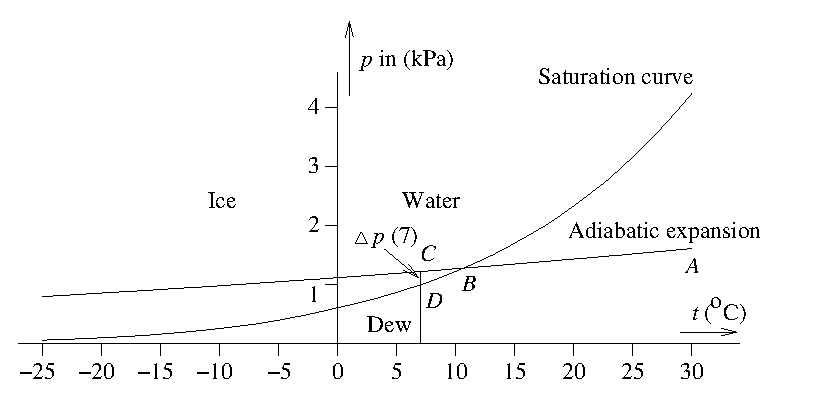
\includegraphics{dew_curve}%
\end{picture}%
\setlength{\unitlength}{4144sp}%
%
\begingroup\makeatletter\ifx\SetFigFont\undefined%
\gdef\SetFigFont#1#2#3#4#5{%
  \reset@font\fontsize{#1}{#2pt}%
  \fontfamily{#3}\fontseries{#4}\fontshape{#5}%
  \selectfont}%
\fi\endgroup%
\begin{picture}(6014,2772)(-2444,554)
\end{picture}%
\caption{Dew curve of water vapour.}\label{fig:dew_curve}
\end{center}\end{figure}

In figure~\ref{fig:dew_curve} the dew point as a function of temperature is plotted. An extra line indicating an adiabatic expansion process going from point A to B and then C is also drawn in this figure. The relative humidity of the gas in this process is obtained by calculating the ratio between the pressure of the gas and the saturation pressure. At point B in the graph is gas is saturated, the relative humidity is 100\%. A further reduction in temperature will yield a gas with a saturation of more than 100\%, a supersaturated gas. The state is unstable. On every irregularity or rough surface the vapour will condense.

In a Wilson chamber these irregularities are created by the charged particles flying through the chamber. The more vapour condenses the clearer the lines drawn by the particles. The amount of condensed mass can be calculated using the ratio between the gas pressure and saturation pressure at the chamber (or gas) temperature. If the chamber is at 7$^\circ$ Celsius this is the ratio of the distance between points C and D and point C figure~\ref{fig:dew_curve}.


\begin{shaded}
\textbf{Exercise \theExercise \stepcounter{Exercise}} : Equation~\ref{eq:gas_c1} allows us to calculate the expansion needed to operate a cloud chamber. According to Wilson the expansion factor needed to be 1.31. How large is the change in pressure with this expansion factor?\end{shaded}

\end{document}


\begin{shaded}
\textbf{Exercise \theExercise \stepcounter{Exercise}} : \end{shaded}

\footnotemark
\footnotetext{}
